\documentclass[11pt,a4paper]{article}

\usepackage[utf8]{inputenc}
\usepackage[T1]{fontenc}
\usepackage[brazil]{babel}
\usepackage{amsmath,amssymb}
\usepackage{newtxtext,newtxmath}
\usepackage{geometry}
\usepackage{fancyhdr}
\usepackage{booktabs}
\usepackage{array}
\usepackage{enumitem}
\usepackage{titlesec}
\usepackage{hyperref}
\usepackage{microtype}
\usepackage{verbatim}
\usepackage{graphicx}

\geometry{margin=2.3cm}
\setlength{\parindent}{1.2em}
\setlength{\parskip}{0.25em}
\setcounter{tocdepth}{2}
\renewcommand{\contentsname}{CONTENTS}

\pagestyle{fancy}
\fancyhf{}
\fancyhead[L]{\textsc{Física Computacional}}
\fancyhead[R]{\textsc{Modelagem de Investimentos}}
\fancyfoot[C]{\thepage}
\renewcommand{\headrulewidth}{0.4pt}

\titleformat{\section}
  {\normalfont\large\bfseries}
  {\thesection}
  {0.7em}
  {\MakeUppercase}

\titleformat{\subsection}
  {\normalfont\normalsize\bfseries}
  {\thesubsection}
  {0.7em}
  {}

\newcommand{\tituloapostila}{
    \begin{center}
        {\LARGE Física Computacional}\\[0.25cm]
        {\Large Investimentos, Modelagem Matemática e Simulação Simples}\\[0.25cm]
        {\normalsize (Dated: 23 de março de 2026)}
    \end{center}
}

\begin{document}
\thispagestyle{plain}
\tituloapostila
\tableofcontents

\section{Introdução}

Esta apostila tem um objetivo simples: introduzir modelos de investimento que sejam
claros o bastante para serem discutidos em sala e fáceis o bastante para serem simulados
em Python. O foco aqui não é reproduzir o mercado financeiro em todos os seus detalhes,
mas construir modelos transparentes, interpretar parâmetros e comparar curvas.

Na linguagem do problema, \(P\) representa o capital acumulado, \(A\) representa o
aporte periódico e \(r\) ou \(i\) representam taxas de rendimento. O interesse didático
desse tema está em três pontos:

\begin{itemize}[leftmargin=*, itemsep=0.2em]
    \item ele produz modelos discretos e contínuos muito simples;
    \item ele permite discutir crescimento linear, composto e não linear;
    \item ele conecta modelagem matemática, simulação e interpretação gráfica.
\end{itemize}

Em uma primeira aproximação, um bom modelo deve ser simples o suficiente para ser
explicado e implementado, mas rico o bastante para distinguir mecanismos diferentes de
crescimento. Neste texto, vamos considerar três situações:

\begin{itemize}[leftmargin=*, itemsep=0.2em]
    \item crescimento linear;
    \item juros compostos com aporte mensal;
    \item crescimento generalizado com o parâmetro \(\alpha\).
\end{itemize}

\section{Modelagem Matemática}

A modelagem matemática reduz um sistema real a um conjunto menor de variáveis e
relações. No caso de investimentos simples, queremos descrever como o capital muda ao
longo do tempo em função do saldo já acumulado, dos novos aportes e da taxa de retorno.

\subsection{Capital, aporte e taxa}

Se \(P_n\) denota o capital no final do mês \(n\), \(A\) denota o aporte mensal e \(i_n\)
denota a taxa aplicada naquele mês, então o modelo discreto mais natural é
\begin{equation}
P_{n+1} = P_n (1+i_n) + A.
\end{equation}

Essa expressão separa claramente os dois mecanismos do problema:
\begin{itemize}[leftmargin=*, itemsep=0.2em]
    \item o termo \(P_n(1+i_n)\) representa a capitalização do saldo;
    \item o termo \(A\) representa o novo dinheiro colocado no sistema.
\end{itemize}

Quando a taxa é constante, temos \(i_n=i\). Quando a taxa muda de ano para ano, basta
trocar \(i_n\) pelo valor correspondente ao bloco temporal em que o mês está inserido.

\subsection{Modelo linear}

Como primeira comparação, pode-se imaginar um modelo em que o ganho por unidade de
tempo é fixo. Nesse caso, o capital cresce como
\begin{equation}
P(t)=P_0 + jt + At,
\end{equation}
onde \(j\) é um ganho constante. Esse modelo gera curvas lineares em função do tempo.
Ele é útil para introduzir a discussão, mas não representa bem a lógica dos juros
compostos, pois o ganho não depende do saldo acumulado.

\subsection{Juros compostos com aporte mensal}

O modelo discreto
\begin{equation}
P_{n+1}=P_n(1+i)+A
\end{equation}
é a forma mais didática de tratar investimento mensal. Ele mostra com clareza o que se
observa na prática: no começo, o crescimento do capital é dominado pelo aporte; em
horizontes maiores, o termo de capitalização passa a ter peso cada vez maior.

Se o aporte é nulo, \(A=0\), recupera-se o caso composto puro:
\begin{equation}
P_{n+1}=P_n(1+i).
\end{equation}

\begin{figure}[h]
\centering
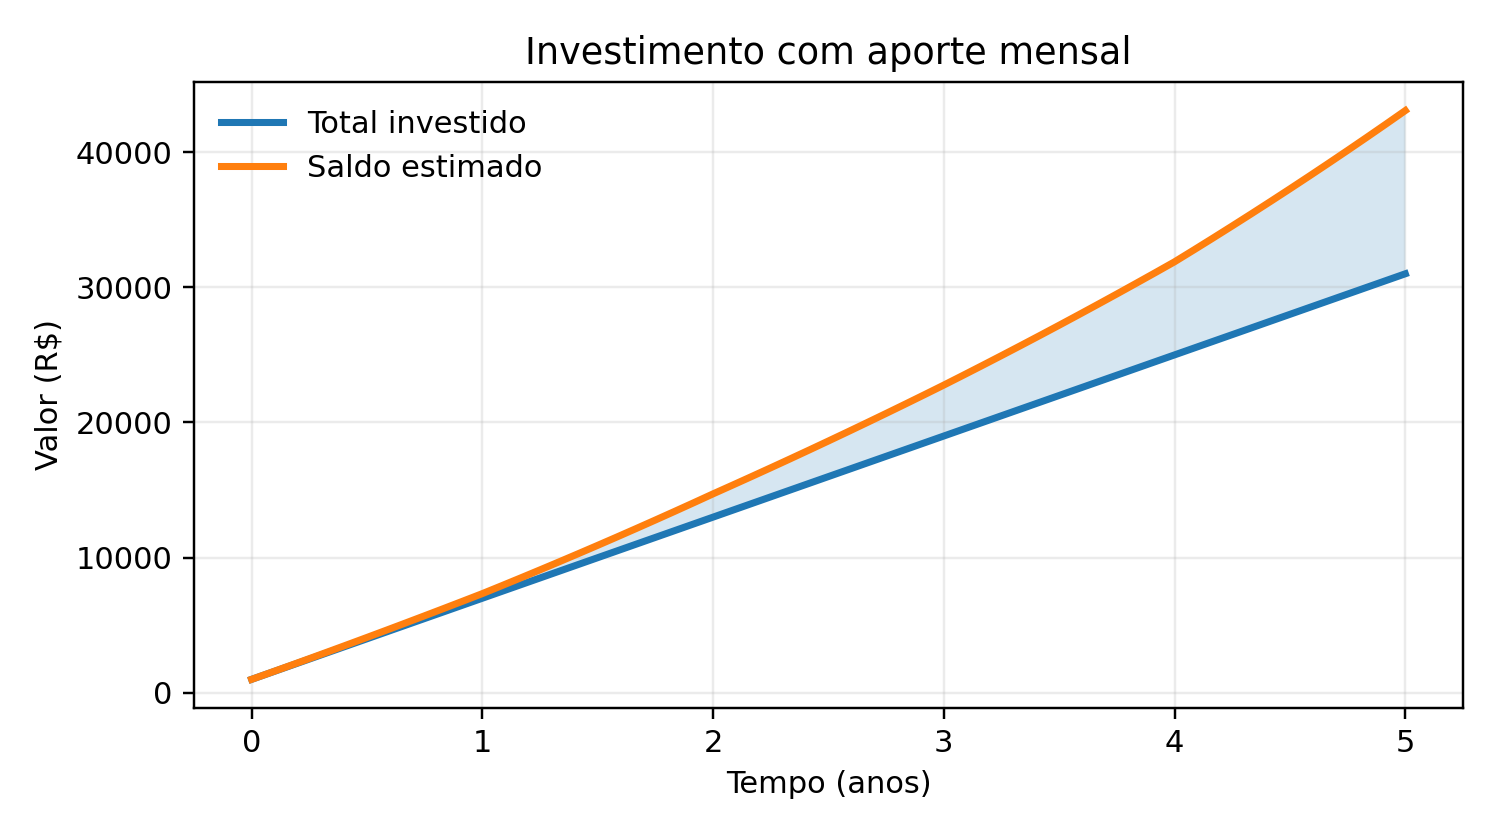
\includegraphics[width=0.78\textwidth]{figuras/investimento_simples.png}
\caption{Exemplo simples de evolução do capital com aporte mensal e taxas anuais por blocos.}
\end{figure}

\subsection{Taxa anual e taxa mensal equivalente}

Em muitos contextos, a taxa de referência é anual. Para implementar uma simulação
mensal, usamos a taxa mensal equivalente
\begin{equation}
i_{\text{mensal}} = (1+r_{\text{anual}})^{1/12} - 1.
\end{equation}

Essa escolha é preferível a uma simples divisão por doze, pois preserva a equivalência
anual do processo composto. Quando se trabalha com uma lista de taxas anuais, como em
um exemplo inspirado na Selic, cada bloco de doze meses pode receber uma taxa anual
própria.

\subsection{Modelo generalizado com \(\alpha\)}

Para comparar regimes de crescimento, consideramos a equação diferencial
\begin{equation}
\frac{dP}{dt} = r P^{\alpha}.
\end{equation}

Esse modelo não deve ser apresentado como a descrição padrão de um investimento real.
Seu papel aqui é outro: comparar matematicamente situações em que o crescimento é
subexponencial, exponencial ou superacelerado.

Para \(\alpha = 1\), a solução é exponencial:
\begin{equation}
P(t)=P_0 e^{rt}.
\end{equation}

Para \(\alpha \neq 1\), obtemos
\begin{equation}
P(t)=\left[P_0^{1-\alpha} + (1-\alpha)rt\right]^{\frac{1}{1-\alpha}}.
\end{equation}

\begin{figure}[h]
\centering
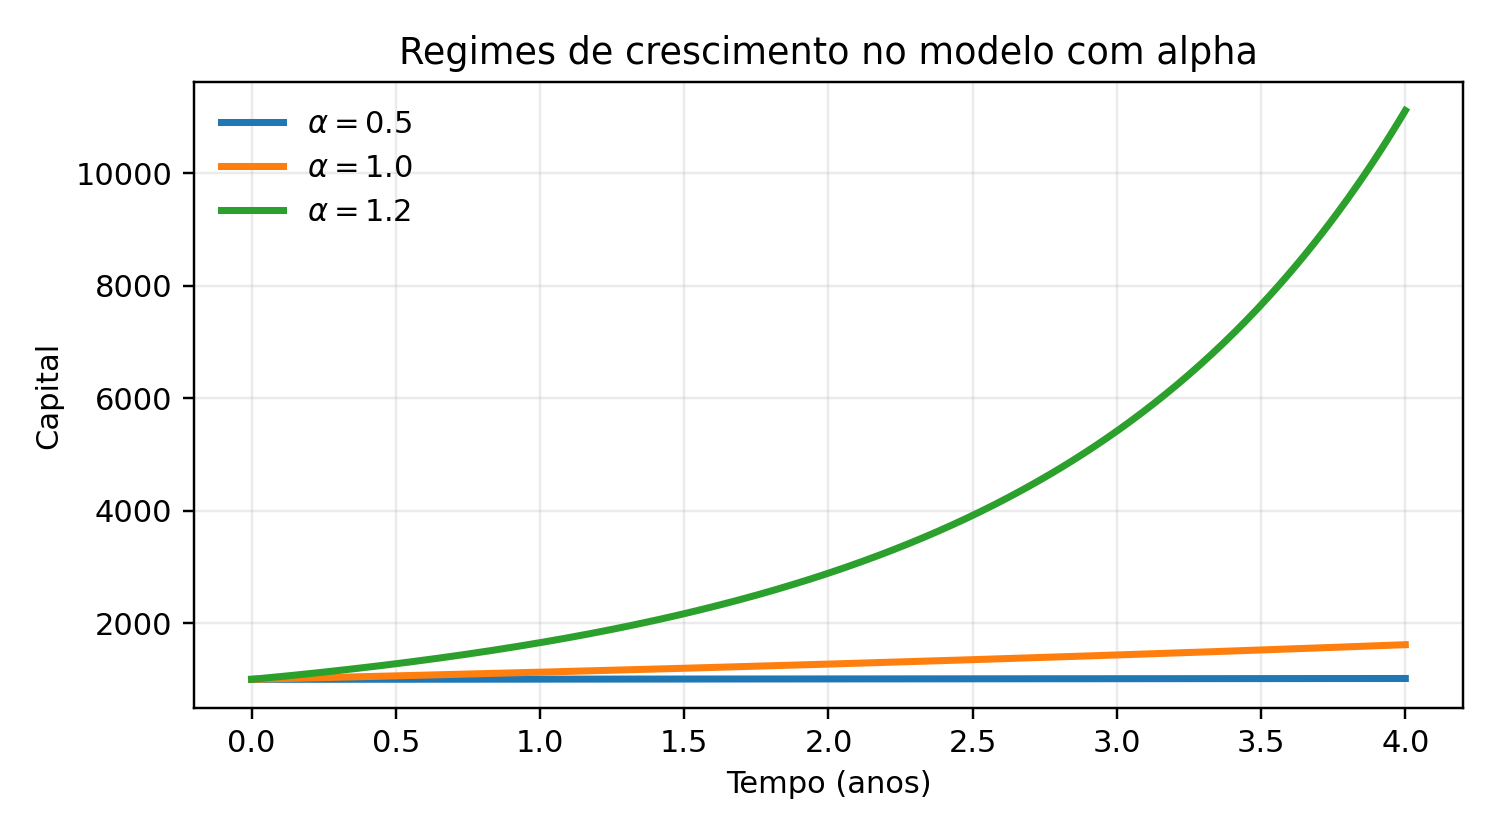
\includegraphics[width=0.78\textwidth]{figuras/regimes_alpha.png}
\caption{Comparação entre os regimes subexponencial, exponencial e superacelerado.}
\end{figure}

\subsection{Regimes de crescimento}

O papel do parâmetro \(\alpha\) pode ser resumido da seguinte maneira:

\begin{center}
\begin{tabular}{>{\raggedright\arraybackslash}p{2.2cm} >{\raggedright\arraybackslash}p{3.8cm} >{\raggedright\arraybackslash}p{5.6cm}}
\toprule
\textbf{Regime} & \textbf{Condição} & \textbf{Interpretação} \\
\midrule
subexponencial & \(\alpha<1\) & o crescimento aumenta com \(P\), mas menos do que proporcionalmente \\
exponencial & \(\alpha=1\) & crescimento proporcional ao capital acumulado \\
superacelerado & \(\alpha>1\) & o crescimento aumenta mais do que proporcionalmente e pode levar a uma explosão em tempo finito \\
\bottomrule
\end{tabular}
\end{center}

No caso \(\alpha>1\) e \(r>0\), a expressão entre colchetes da solução pode zerar em um
tempo finito. Isso define um limite teórico para o domínio da solução:
\begin{equation}
t_c = \frac{P_0^{1-\alpha}}{(\alpha-1)r}.
\end{equation}

\subsection{Qualidade do modelo}

Ao construir um modelo, convém perguntar:
\begin{itemize}[leftmargin=*, itemsep=0.2em]
    \item quais variáveis realmente importam para o problema;
    \item quais detalhes foram descartados;
    \item até que ponto a simplificação ainda preserva a interpretação desejada.
\end{itemize}

No contexto desta apostila, deixamos de fora custos, impostos, inflação, risco,
marcação a mercado e incerteza estocástica. Isso não é um defeito do modelo inicial.
É uma escolha didática para isolar o mecanismo principal de crescimento.

\section{Aspectos Computacionais}

Do ponto de vista computacional, a implementação mais direta é uma simulação mês a
mês. O algoritmo precisa apenas de vetores para o tempo, o saldo acumulado e o total
investido, além de um laço que atualize o capital.

\subsection{Algoritmo mínimo}

Um núcleo de código suficientemente curto para a primeira versão é:

\begin{verbatim}
for mes in range(meses):
    indice_ano = min(mes // 12, len(taxas) - 1)
    taxa_mensal = (1 + taxas[indice_ano]) ** (1/12) - 1
    saldo[mes + 1] = saldo[mes] * (1 + taxa_mensal) + aporte
    investido[mes + 1] = investido[mes] + aporte
\end{verbatim}

Esse algoritmo fornece duas curvas particularmente úteis:
\begin{itemize}[leftmargin=*, itemsep=0.2em]
    \item o total investido pelo usuário;
    \item o saldo estimado com capitalização.
\end{itemize}

A distância entre essas curvas representa o rendimento bruto acumulado no modelo.

\subsection{Entradas e saídas}

Para a primeira versão didática, basta pedir ao usuário:
\begin{itemize}[leftmargin=*, itemsep=0.2em]
    \item capital inicial;
    \item aporte mensal;
    \item tempo total da simulação.
\end{itemize}

As taxas anuais podem ficar definidas no próprio código. As saídas mínimas mais úteis são:
\begin{itemize}[leftmargin=*, itemsep=0.2em]
    \item valor final do capital;
    \item total investido;
    \item rendimento bruto;
    \item gráfico do saldo estimado e do total investido.
\end{itemize}

\subsection{Interpretação dos gráficos}

Em horizontes curtos, o crescimento do saldo costuma acompanhar de perto a curva do
total investido. Em horizontes mais longos, a distância entre as curvas aumenta e o papel
da capitalização se torna evidente. No modelo com \(\alpha\), a análise gráfica é ainda
mais rica, pois podemos comparar:

\begin{itemize}[leftmargin=*, itemsep=0.2em]
    \item o gráfico de \(P(t)\), que mostra a evolução temporal;
    \item o gráfico de \(dP/dt\) em função de \(P\), que mostra a lei de crescimento.
\end{itemize}

Esse segundo gráfico funciona como um diagrama de fase simples: ele informa como a taxa
instantânea de crescimento depende do próprio capital.

\section{Exercícios}

\begin{enumerate}[leftmargin=*, itemsep=0.8em]
    \item Use \(P_0=1000\) reais, \(A=500\) reais por mês e horizonte de \(5\) anos.
    Implemente o algoritmo mensal com uma sequência anual de taxas e faça o gráfico do
    saldo estimado e do total investido.

    \item Repita a simulação anterior para \(A=250\), \(500\) e \(1000\) reais. Compare os
    valores finais e discuta em qual faixa de tempo o aumento do aporte é mais relevante.

    \item Fixe o aporte mensal e o tempo total. Varie apenas o capital inicial e analise como
    isso afeta o valor final. Discuta por que o efeito de \(P_0\) cresce com o horizonte de
    tempo.

    \item Mostre numericamente a diferença entre usar
    \(i_{\text{mensal}} = r_{\text{anual}}/12\) e
    \(i_{\text{mensal}} = (1+r_{\text{anual}})^{1/12}-1\). Discuta qual escolha é mais
    coerente para capitalização composta.

    \item Implemente um modelo linear simples e compare-o com o modelo composto usando os
    mesmos valores de entrada. Faça um gráfico com as duas curvas e identifique quando a
    diferença entre elas se torna significativa.

    \item Considere a equação \(dP/dt = rP^{\alpha}\) com \(P_0>0\) e \(r>0\). Plote as
    curvas para \(\alpha = 0.5\), \(\alpha = 1.0\) e \(\alpha = 1.2\), mantendo os demais
    parâmetros fixos. Compare os três regimes.

    \item A partir da solução analítica do modelo com \(\alpha\), determine o tempo crítico
    \(t_c\) quando \(\alpha>1\). Verifique numericamente o que acontece com a curva ao se
    aproximar desse limite.

    \item Escolha valores de \(\alpha\) cada vez mais próximos de \(1\) e compare a solução
    generalizada com a solução exponencial. Faça um gráfico do erro relativo em função de
    \(\alpha\).

    \item Construa o gráfico de \(dP/dt\) em função de \(P\) para diferentes valores de
    \(\alpha\). Explique como a inclinação e a curvatura do diagrama ajudam a interpretar o
    tipo de crescimento.

    \item Proponha uma extensão do código que permita escolher uma data inicial e aplicar
    taxas anuais diferentes ao longo do tempo. Descreva como você adaptaria o modelo para
    um cenário inspirado na Selic ou em um CDB indexado ao CDI.
\end{enumerate}

\end{document}
